\chapter[SCP-171 集合脑泡沫]{
    SCP-171 Collective Brain Foam\\
    SCP-171 集合脑泡沫
}

\label{chap:SCP-171}

\begin{figure}[H]
    \centering
    
\includegraphics[width=0.5\linewidth]{images/SCP-171.jpg}
    \caption*{初见SCP-171}
\end{figure}

\bb{项目编号:}SCP-171

\bb{项目等级:}Euclid

\bb{特殊收容措施:}目前在对SCP-171进行研究的地点是位于生化研究区-12的一个容量为4500公升的海水池。虽然不会立即产生危害,但是尽可能不要与SCP-171的主体及分泌物直接接触。主体与研究员之间的一切交流都必须被录音及抄录下来。对于人类主体则将投喂素食以供选择。对其他动物主体也将进行适当的饲喂。必须在水池中定期循环新鲜海水。

\bb{描述:}起初,SCP-171被认为是与\hyperref[chap:SCP-968]{SCP-968}或\hyperref[chap:SCP-165]{SCP-165}类似的微生物菌落,但是进一步调查显示初次发现时SCP-171是覆盖范围超过300平方米的单个实体。SCP-171是由细小的神经元卷须、粘液腺和悬浮在它自己制造的泡沫中的肌纤维组成的网状母体。它不能自己移动,不会主动攻击,也不以其他活的生物体为食;恰恰相反,它试图与它遇到的所有生物体形成共生关系。

\begin{figure}[H]
    \centering
    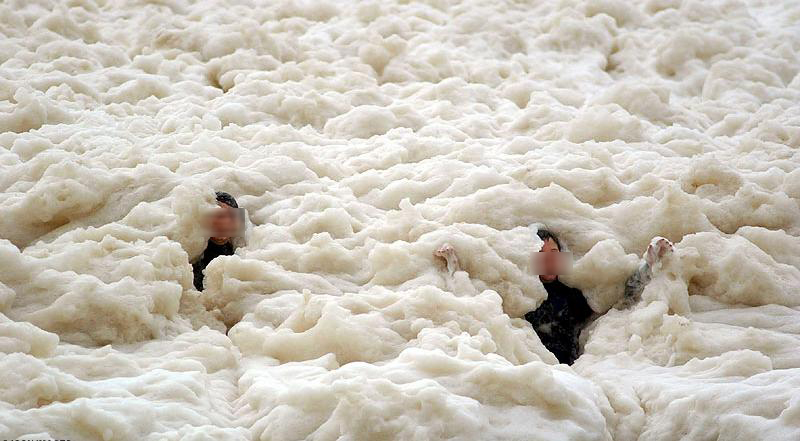
\includegraphics[width=0.5\linewidth]{images/SCP-171-2.jpg}
    \caption*{在被整合前不久于SCP-171的泡沫中玩耍的儿童}
\end{figure}

环绕在神经纤维四周的肌肉的鞭毛将黏液、海盐、水及其他分泌物做成泡状,形成一个巨大的泡沫支架。任何花大把时间接触SCP-171母体的生物都有被整合进由它供养的集体意识之中的危险。被SCP-171所覆盖的人形容说经历了一阵“刺痛”或是“酥痒”感,研究者在此过程中观察到SCP-171的线钻进皮肤直接整合进对象的神经系统中。一段时间后,对象的基本运动神经元发展成为精细复杂的双向交流系结,使主体的脑部能互相交流,也能与SCP-171的实体交流。久而久之,对象的个人特征将与SCP-171母体的其他人整合与共享,最终成为不存在个性的集体意志。

目前SCP-171上有19个人类主体(11个平民,8个D级人员)。主体皮肤上形成了能允许主体和SCP-171以神经末梢与脑内树突相同的方式进行化学通信,使主体能够在不与集合体断开连接的情况下穿过泡沫的神经受体。皮肤上的这些受体看上去像是介于白色与透明色之间的痣,微微凸起,对碰触非常敏感。有些主体在SCP-171中消失长达数月。他们在没有淡水和食物的情况下存活的方式未知。

\begin{figure}[H]
    \centering
    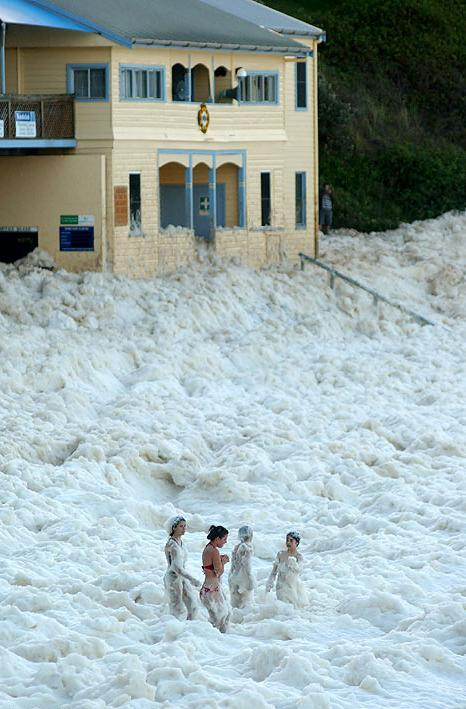
\includegraphics[width=0.5\linewidth]{images/SCP-171-3.jpg}
    \caption*{最初,整个海岸线地带都被泡沫覆盖了}
\end{figure}

其他主体包括:2只澳大利亚鼠海豚(最初有4只),4只海鸥(3只已被安乐死),41条各种品种的鱼(为进行研究已被安乐死),27只滨蟹(为进行研究已被安乐死),以及一只狗。在2小时内,大部分的主体就开始在皮肤上形成神经受体,并且接收到来自SCP-171的神经联系了。3小时以后,主体和集合体之间就已经建立起精神上的联系了。6小时之后,对集合体发展出了完全的统和与依赖关系。在这个时候,断开主体与SCP-171的联系会导致主体处于狂躁状态,并使主体表现出暴力行为,最终导致主体精神崩溃,进入植物人状态(有四个人变成了这样)。

当接受采访的时候,所有的主体就像是一个主体的组成部分一样以同核的集体意识说话。集合体清楚地意识到自己的存在,而且对于自己中存在着不同的人这一事实十分镇静,甚至会对每个损失的主体表示哀悼之情。SCP-171告诉研究员它很明白它是什么,但是不知道它是从哪来的,并且解释说由于它自己和它包含的主体的智能太愚钝了,它们无法理解或是记忆它的来源。研究员注意到在整合进d级人员之后SCP-171的性格发生了变化,决定从此以后不能让它整合内心充满暴力、怨恨或是恶意的人员。SCP-171通过沉思和理解之后表示,它决定尽可能不食用动物。

\bb{附录171-1} 2007年8月12日,海滩游客和冲浪者在澳大利亚海岸线近新南威尔士州Yamba地区首次遇见SCP-171。当平民在泡沫中玩耍的时候皮肤状况开始出现异常,疾病防治中心官员无法解释此异常现象,于是联系了SCP基金会人员。

\bb{附录171-2} 自愿被整合进SCP-171共同体的人必须先通过一个全方位心理测试来确保良好的心理健康状态,心理测试特别强调失去人性的可能性以及潜在的自杀倾向。将会多次警告他们这种整合是永久性的,而且没有证据证明SCP-171表现出了“高觉悟”的状态,或是与我们自己的意识有什么显著的不同。如果有人坚持希望被整合,并且是在心智健全的状况下做出这种决定的,那么允许他们去实现愿望。
